%%%%%%%%%%%%%%%%%%%%%%%%%%%%%%%%%%%%%%%%%%%%%%%%%%%%%%%%%%%%%%%%%%%%%%%%%%%%%%%%%%%%%%%%%%%%%%%%
%
% CS576 Written Question Template
%
% Acknowledgements:
% The original code is written by Prof. James Tompkin (james_tompkin@brown.edu).
% The second version is revised by Prof. Min H. Kim (minhkim@kaist.ac.kr).
%
% This is a LaTeX document. LaTeX is a markup language for producing 
% documents. Your task is to fill out this document, then to compile 
% it into a PDF document. 
%
% 
% TO COMPILE:
% > pdflatex thisfile.tex
%
% If you do not have LaTeX and need a LaTeX distribution:
% - Personal laptops (all common OS): www.latex-project.org/get/
% - We recommend latex compiler miktex (https://miktex.org/) for windows,
%   macTex (http://www.tug.org/mactex/) for macOS users.
%   And TeXstudio(http://www.texstudio.org/) for latex editor.
%   You should install both compiler and editor for editing latex.
%   The another option is Overleaf (https://www.overleaf.com/) which is 
%   an online latex editor.
%
% If you need help with LaTeX, please come to office hours. 
% Or, there is plenty of help online:
% https://en.wikibooks.org/wiki/LaTeX
%
% Good luck!
% Min and the CS576 staff
%
%%%%%%%%%%%%%%%%%%%%%%%%%%%%%%%%%%%%%%%%%%%%%%%%%%%%%%%%%%%%%%%%%%%%%%%%%%%%%%%%%%%%%%%%%%%%%%%%
%
% How to include two graphics on the same line:
% 
% \includegraphics[\width=0.49\linewidth]{yourgraphic1.png}
% \includegraphics[\width=0.49\linewidth]{yourgraphic2.png}
%
% How to include equations:
%
% \begin{equation}
% y = mx+c
% \end{equation}
% 
%%%%%%%%%%%%%%%%%%%%%%%%%%%%%%%%%%%%%%%%%%%%%%%%%%%%%%%%%%%%%%%%%%%%%%%%%%%%%%%%%%%%%%%%%%%%%%%%

\documentclass[11pt]{article}

\usepackage[english]{babel}
\usepackage[utf8]{inputenc}
\usepackage[colorlinks = true,
            linkcolor = blue,
            urlcolor  = blue]{hyperref}
\usepackage[a4paper,margin=1.5in]{geometry}
\usepackage{stackengine,graphicx}
\usepackage{fancyhdr}
\setlength{\headheight}{15pt}
\usepackage{microtype}
\usepackage{times}
\usepackage{booktabs}

% From https://ctan.org/pkg/matlab-prettifier
\usepackage[numbered,framed]{matlab-prettifier}

\frenchspacing
\setlength{\parindent}{0cm} % Default is 15pt.
\setlength{\parskip}{0.3cm plus1mm minus1mm}

\pagestyle{fancy}
\fancyhf{}
\lhead{Homework Writeup}
\rhead{CS576}
\rfoot{\thepage}

\date{}

\title{\vspace{-1cm}Homework 1 Writeup}


\begin{document}
\maketitle
\vspace{-3cm}
\thispagestyle{fancy}

\section*{Instructions}
\begin{itemize}
  \item Describe any interesting decisions you made to write your algorithm.
  \item Show and discuss the results of your algorithm.
  \item Feel free to include code snippets, images, and equations.
  \item There is no page limit.
  
\end{itemize}

\section*{In the beginning...}

Lorem ipsum dolor sit amet, consectetur adipisicing elit, sed do eiusmod tempor incididunt ut labore et dolore magna aliqua. Ut enim ad minim veniam, quis nostrud exercitation ullamco laboris nisi ut aliquip ex ea commodo consequat. Duis aute irure dolor in reprehenderit in voluptate velit esse cillum dolore eu fugiat nulla pariatur. Excepteur sint occaecat cupidatat non proident, sunt in culpa qui officia deserunt mollit anim id est laborum. See Equation~\ref{eq:one}.

\begin{equation}
a = b + c
\label{eq:one}
\end{equation}

\section*{Interesting Implementation Detail}

\begin{lstlisting}[style=Matlab-editor]
for k = 1:numView
    [~, ~, V] = svd(L(:,:,k));
    h = V(:,9);
    h = h / h(9);
    homography(:,:,k) = reshape(h, [3,3])';
end
\end{lstlisting}

In homography calculation part, I calculate smallest right singular vector of L and normalize h33 to be 1, at each view



\begin{lstlisting}[style=Matlab-editor]
function [objective] = func_calibration(imagePoints, worldPoints, x)
    
numView = size(imagePoints,3);
hat_m = zeros(size(imagePoints));

% ----- Your code here (9) -----

K = [1, 0, 0
     0, 1, 0
     0, 0, 1];
 
K(1,1) = x(1);
K(1,2) = x(2);
K(1,3) = x(3);
K(2,2) = x(4);
K(2,3) = x(5);

for view = 1:numView
    rvec = x(6*view+3:6*view+5);
    tvec = x(6*view:6*view+2);
    R = rotationVectorToMatrix(rvec);
    R = R';
    P = K * [R(:,1), R(:,2), reshape(tvec,[3,1])];
    points = worldPoints;
    points = [points, ones(size(imagePoints,1), 1)];
    hat = P * points';
    hat(1,:) = hat(1,:) ./ hat(3,:);
    hat(2,:) = hat(2,:) ./ hat(3,:);
    hat_m(:,:,view) = hat(1:2,:)';
end

objective = imagePoints - hat_m;
\end{lstlisting}

In optimizing function used to MLE, first, I reconstruct K and Projection matrix from x. Then I add ones vector to worldPoints matrix, because of making homogenious coord. And I calcuate q(hat)ij.

\begin{lstlisting}[style=Matlab-editor]
cost_vol = zeros(m, n, max_disparity);

pad_right = padarray(rightImageGray, [0 max_disparity], 'replicate', 'pre');

block_pad = round(w/2) - 1;

pad_left = padarray(leftImageGray,[block_pad block_pad], 'replicate', 'both');
padded_right = padarray(pad_right, [block_pad block_pad], 'replicate', 'both');


filter = zeros(w);
filter(1:w, 1:w) = 1 / (w^2);

avg_right = imfilter(pad_right, filter, 'replicate');
avg_left = imfilter(leftImageGray, filter, 'replicate');

for i=1:m
    for j=1:n
        for d = 1:max_disparity
            j2 = j -d + max_disparity;
            avg_l = avg_left(i, j);
            avg_r = avg_right(i,j2);
            A = pad_left(i:i+w-1, j:j+w-1);
            a = A(:) - avg_l;
            B = padded_right(i:i+w-1, j2:j2+w-1);
            b = B(:) - avg_r;
            cost_vol(i,j,d) = -dot(a,b) / (norm(a) * norm(b));
        end
    end
end
\end{lstlisting}

In cost volume with a cost function and cost aggregation part, first, because of boundary I do padding image, then I used average filter to calculate average of all [window size *window size] subarray first. These average values are used when get NCC score. NCCscore’s range is [-1, 1]. When NCC score is 1, I can say this is matched. So I multiple -1to NCC score for change min score mean matching

\begin{lstlisting}[style=Matlab-editor]
cost_vol2 = zeros(m, n, max_disparity);
parent = zeros(m, n, max_disparity);
min_dis = 10;
dis = min_dis:max_disparity;
dis_size = max_disparity - min_dis + 1;

rob = @(x) x.^2 ./ (1 + x.^2);
cost_vol2(:,n,:) = cost_vol(:,n,:);
for i=1:m
    for j=n-1:-1:1
        for d = min_dis:max_disparity
            r = rob(d - dis);
            cost = reshape(cost_vol2(i,j + 1,min_dis:max_disparity), [dis_size, 1])  ...
                + reshape(r, [dis_size, 1]);
            [value, idx] = min(cost);
            cost_vol2(i,j,d) = cost_vol(i,j,d) + value;
            parent(i,j,d) = idx + min_dis - 1;
        end
    end
end
[~, idx] = min(cost_vol2(:,1,min_dis:max_disparity),[],3);
for i=1:m
    disparityMap(i,1) = idx(i) + min_dis - 1;
    idx_next = parent(i,1,idx(i) + min_dis - 1);
    for j=2:n
        disparityMap(i,j) = idx_next;
        idx_next = parent(i,j,idx_next);
    end
end
\end{lstlisting}

In constructing Disparity map part, I use Energy minimization and Dynamic Programming algorithm learned in class, and described below. First triplication for loop is the process of updating the entire cost volume using DP algorithm that considers the disparity of the neighboring pixels, and second double for loop is the process of backtracking which disparity should be given to each pixel.

\begin{figure}[h]
    \centering
    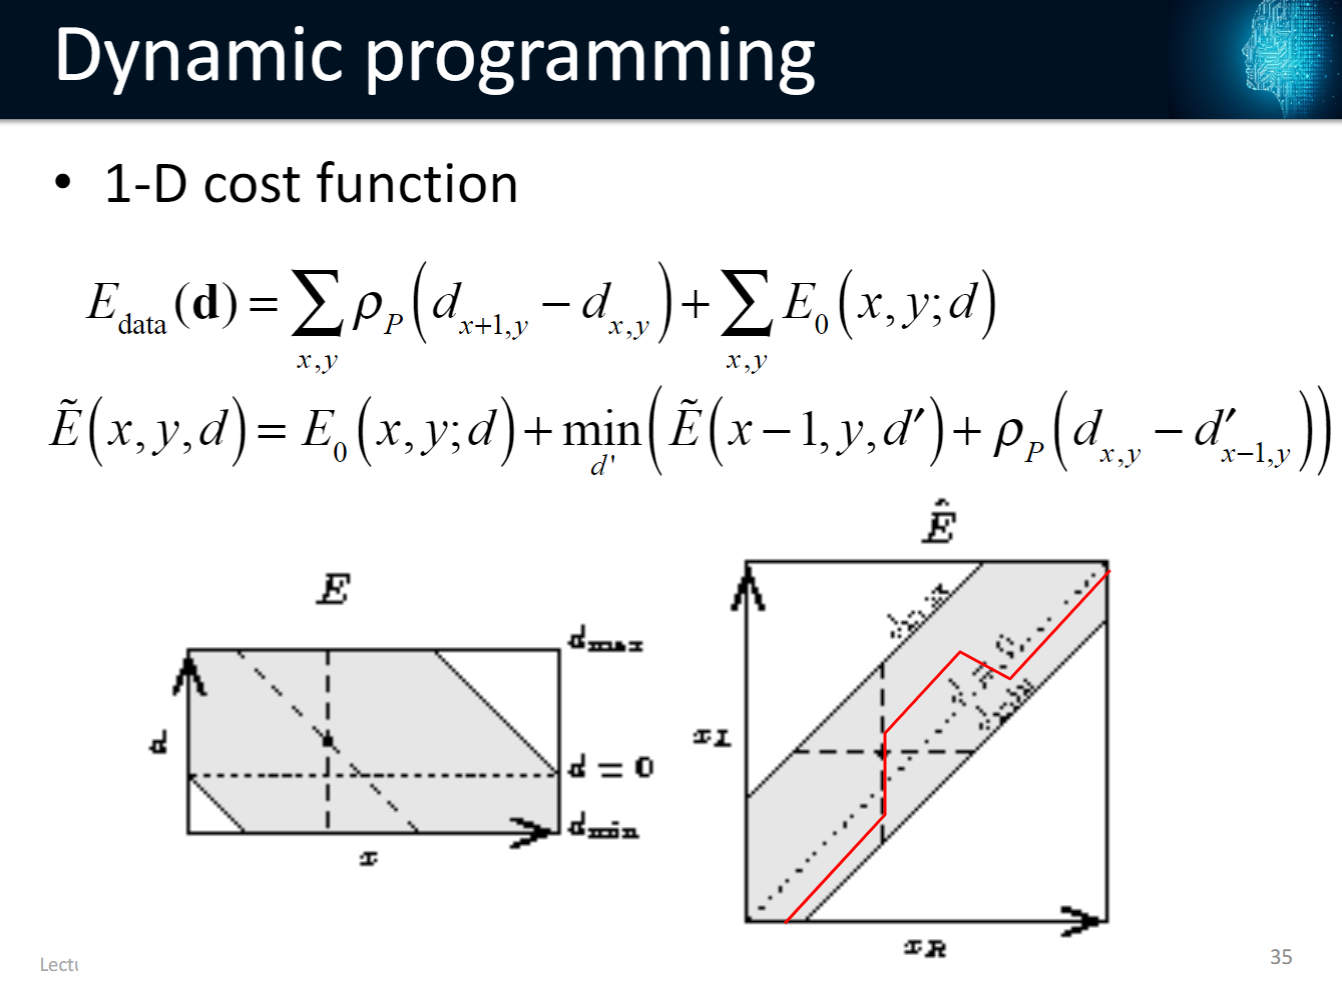
\includegraphics[width=10cm]{algorithm.png}
    \caption{ Energy minimization + DP algorithm}
    \label{fig:result1}
\end{figure}

\pagebreak
\section*{A Result}

\begin{figure}[h]
    \centering
    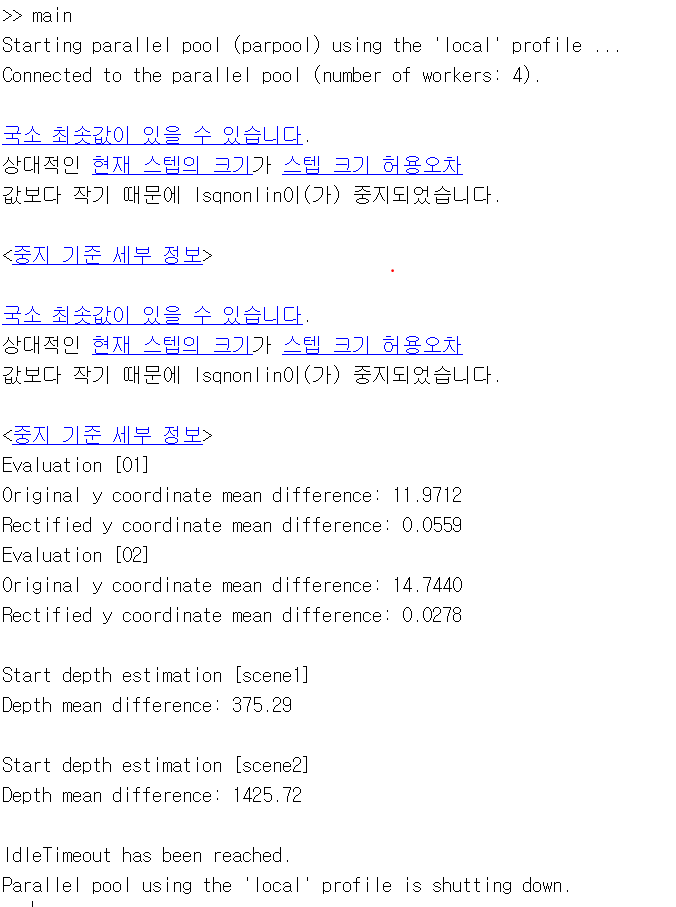
\includegraphics[width=10cm]{result1.png}
    \caption{Output result of entire code}
    \label{fig:result1}
\end{figure}

\pagebreak
\begin{figure}[h]
    \centering
    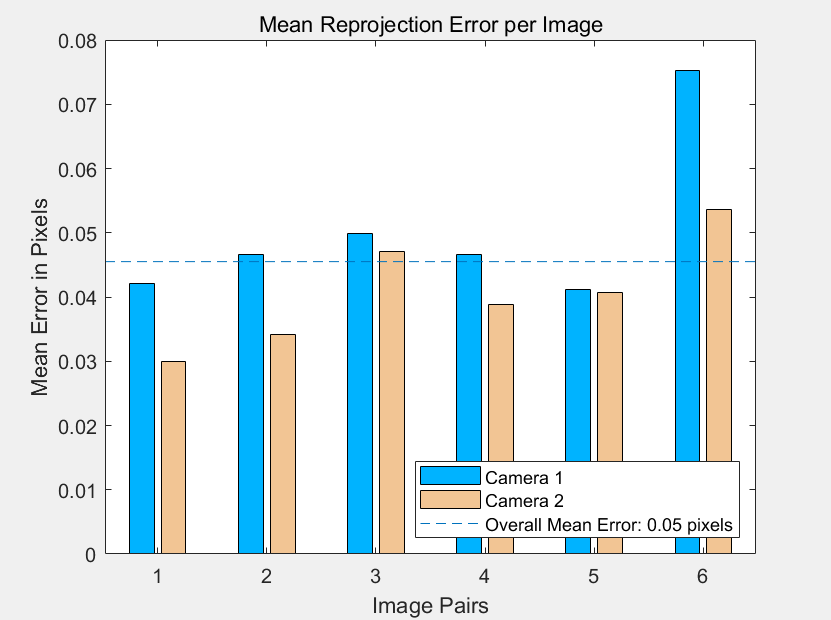
\includegraphics[width=8cm]{result2.png}
    \caption{Reprojection error of camera parameters}
    \label{fig:result1}
\end{figure}

\begin{figure}[h]
    \centering
    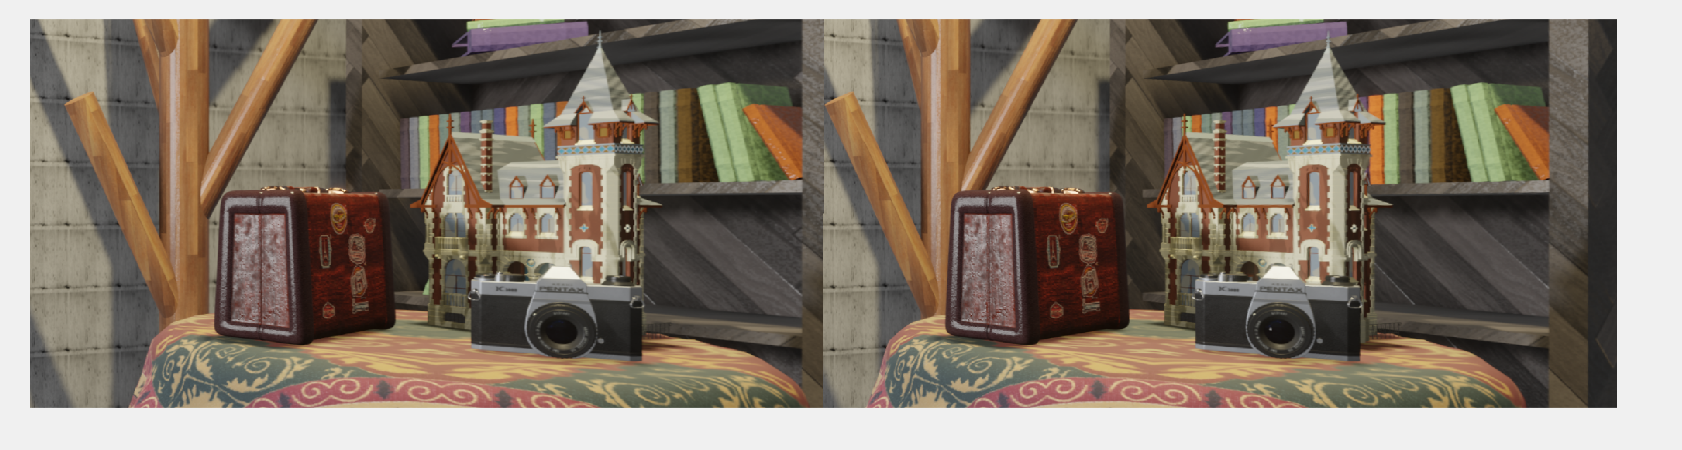
\includegraphics[width=12cm]{result3.png}
    \caption{Reprojection result of scene1}
    \label{fig:result1}
\end{figure}

\begin{figure}[h]
    \centering
    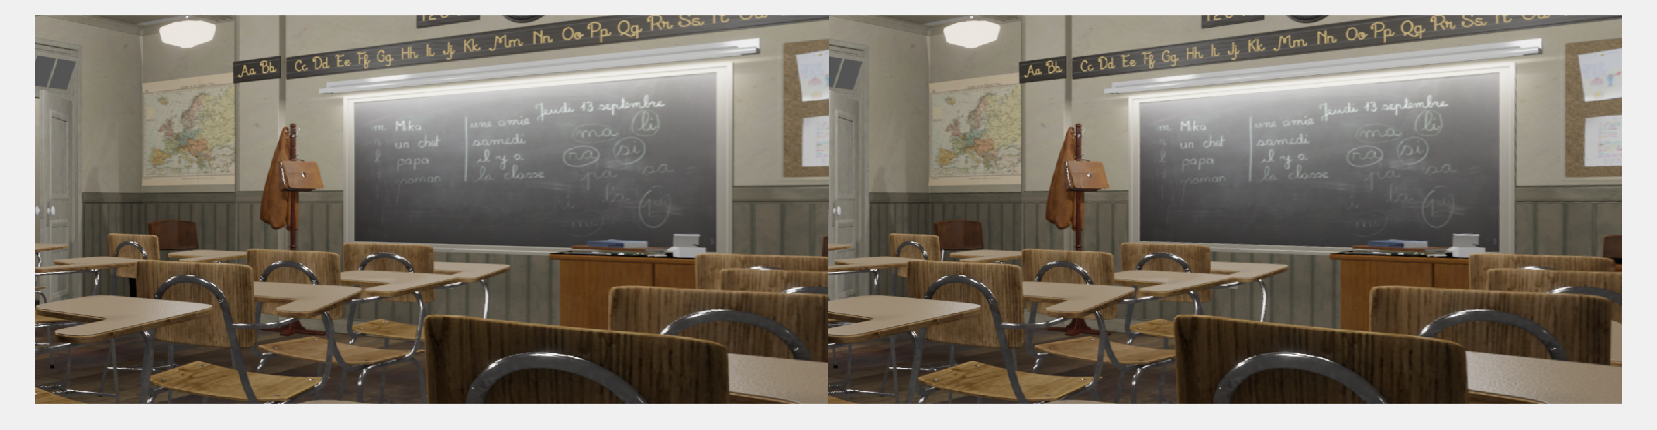
\includegraphics[width=12cm]{result6.png}
    \caption{Reprojection result of scene2}
    \label{fig:result1}
\end{figure}


Reprojection error is 0.0x pixel units, so it can be said it I got very good result. I guess that some error can be caused by inaccuracy of input value and svd function.


\pagebreak
\begin{figure}[h]
    \centering
    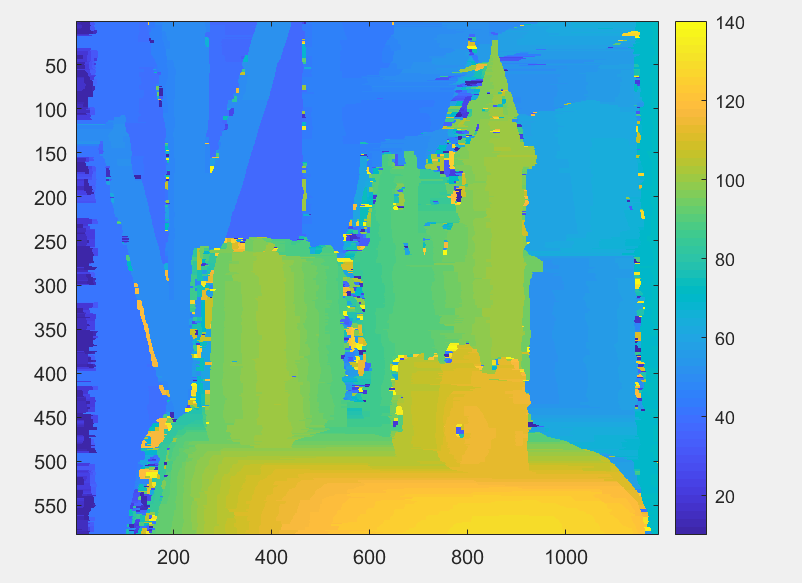
\includegraphics[width=10cm]{result4.png}
    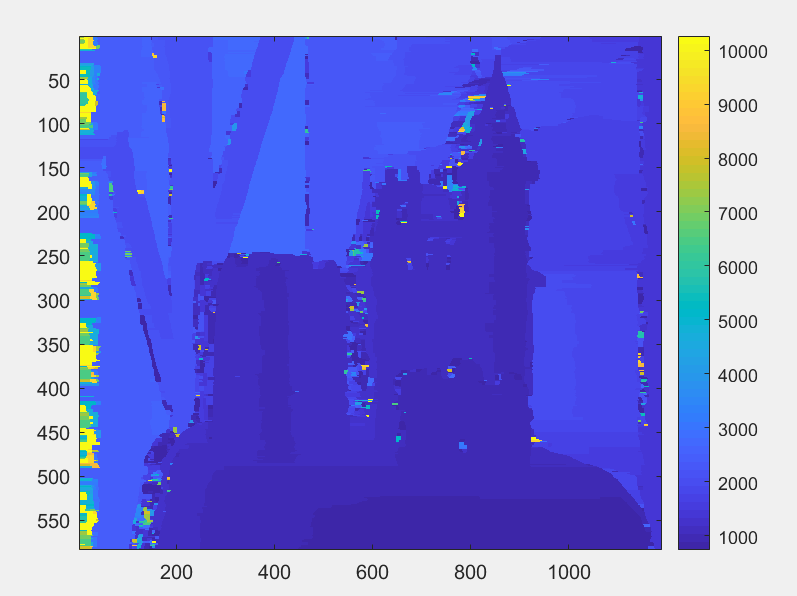
\includegraphics[width=10cm]{result5.png}
    \caption{up : disparity image of scene1, down : depth image of scene1}
    \label{fig:result1}
\end{figure}
\pagebreak
\begin{figure}[h]
    \centering
    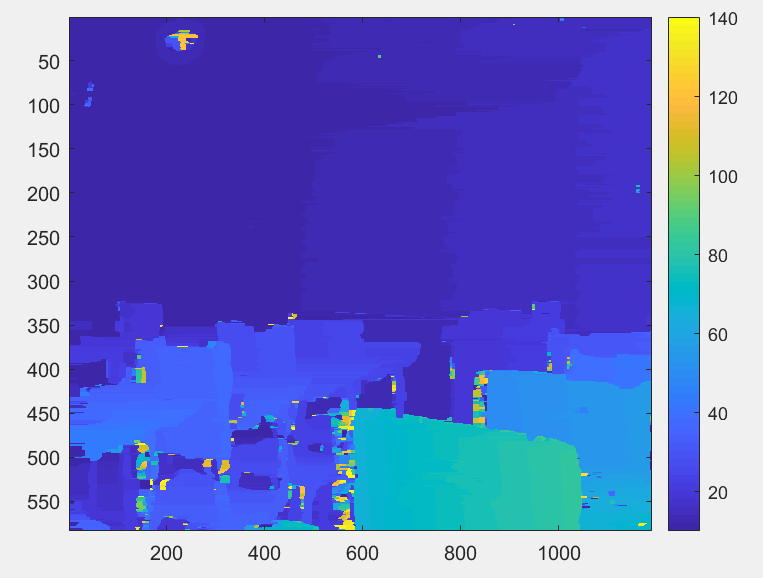
\includegraphics[width=10cm]{result7.png}
    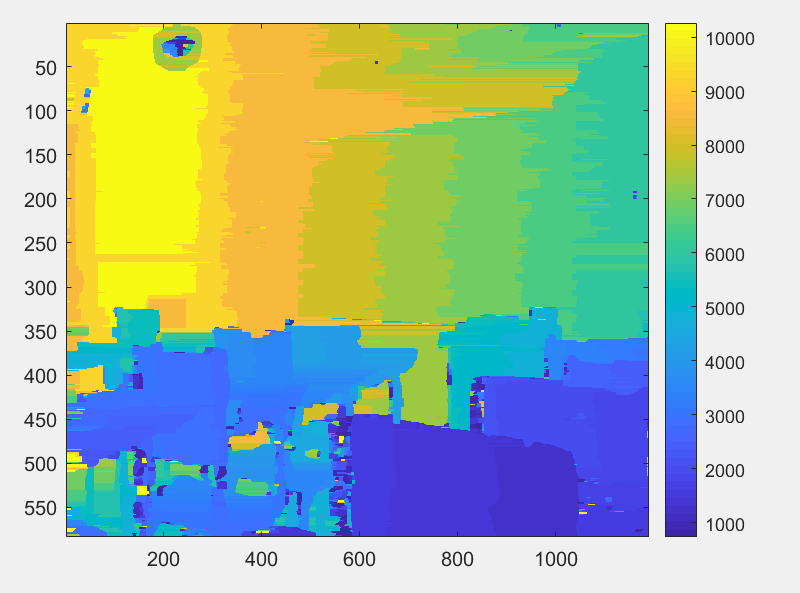
\includegraphics[width=10cm]{result8.png}
    \caption{up : disparity image of scene2, down : depth image of scene2}
    \label{fig:result1}
\end{figure}

I think error of disparity and depth can be caused by lack of parameter tuning and boundary condition. In addition, when low disparity case, small error of disparity cause large error of depth , so there was a high error on the part of the blackboard with relatively low disparity.


\end{document}